% Sean T. Hayes
\documentclass[14pt,aspectratio=1610, hyperref={pdfpagelayout=SinglePage}]{beamer}
%\documentclass[12pt,aspectratio=1610,handout]{beamer}
\usepackage{csu-theme}
\usepackage{linked-lists}
\usepackage{booktabs}

\title{\Huge{} Singly-Linked Lists}
\subtitle{CSCI 315: Data Structure Analysis\\Chapter 16}
\author{Sean T. Hayes, Ph.D.}
\institute{Charleston Southern University}

%% Comment out date to use default (today)
% \date{February 6, 2025}
\subject{Data Structures and Algoirthms}
%\keywords{}

\setlength{\parskip}{0.5em}

\begin{document}

\begin{frame}
  \titlepage{}
\end{frame}

\section{Introduction}

\begin{frame}{Introduction}
\begin{itemize}
\item
  Often, data is organized and processed sequentially (in a \emph{sequential list}).
\item
  An array is a useful data structure for sequential processing, but has its limitations.
  \begin{itemize}
  \item
    Array sizes are fixed.
  \item
    Searching is slow for unsorted arrays.
  \item
    Insertion and deletion are slow because they require data movement.
  \end{itemize}
\end{itemize}
\end{frame}

\begin{frame}{Array Performance}
What is the order of approximation (Big O) of the following operations on an array?
\begin{tabular}{r c}
\toprule
                               & \textbf{Array}\\
\midrule
  Element Access               & \onslide<2->{$O(1)$} \\
  Insert/Remove from Beginning & \onslide<3->{$O(n)$} \\
  Insert at the End       & \onslide<4->{$O(1)$, but $O(n)$ if full} \\
  Remove from End       & \onslide<5->{$O(1)$ with wasted space} \\
  Insert/Remove from Middle    & \onslide<6->{$O(n)$} \\
  Unsorted Search              & \onslide<7->{$O(n)$} \\
\bottomrule
\end{tabular}
\end{frame}

\begin{frame}{Linked Lists}
\begin{itemize}
\item
  \emph{Linked lists} store data in \emph{nodes}, where each node \\contains
  the data and a pointer to the next node.
\item
  The first node is called the head, and the last is the tail.
\end{itemize}
\center%
\begin{tikzpicture}
  \LinkedList[tail]{a,b,c,d,e}
  % \LinkPtr{pHead}
  % \LinkedNode{a}
  % \LinkedNode{b}
  % \LinkedNode{c}
  % \LinkedNode{d}
  % \LinkedNode{e}
  % \TailPtr{pTail}

\end{tikzpicture}
\end{frame}

\begin{frame}{Advantages of Linked Lists}
\begin{itemize}
\item
  A variable size; memory is allocated and released \\as needed.
\item
  Some algorithms are faster with linked lists compared to arrays.
\item
  Expandable to nonlinear data structures (nodes with multiple pointers).\\
  For example, trees and graphs.
\end{itemize}
\end{frame}

\begin{frame}{Disadvantages of Linked Lists}
\begin{itemize}
\item
  Additional memory. Each pointer requires an \\additional 4 or 8 bytes, which may be significant \\with large data sets.
\item
  Discontiguous memory (spread over disconnected locations).
\item
  Some algorithms are slower on Linked Lists, compared to on arrays.
\end{itemize}
\end{frame}

\section{Nodes}

\begin{frame}[fragile]{The \texttt{Node} Class/Struct}
Each node contains a data value (datum) and a pointer to the next node.

\begin{lstlisting}
struct Node {
  Node (const char &value = ' ')
    : datum{value},
      pNext{nullptr}
  {}

  char datum; // holds a value in the list
  Node* pNext;
}
\end{lstlisting}
\end{frame}

\begin{frame}[fragile]{Working with Nodes}
\begin{itemize}
\item<1->
    Variable declaration:\\
    \lstinline|Node *pHead{nullptr};|
\item<3->
    Add a value:\\
    \lstinline|pHead = new Node{'A'};|
\item<5->%
    Add another value:\\
    \lstinline|pHead->pNext = new Node{'B'};|
\item<7->
  Add a third value:\\
  \lstinline|pHead->pNext->pNext = new Node{'C'};|\\
\end{itemize}
\center{}
\begin{tikzpicture}
\onslide<2->{
  \LinkPtr{pHead}
}
\onslide<4->{
  \LinkedNode{\textquotesingle{}A\textquotesingle{}}
}
\onslide<6->{
  \LinkedNode{\textquotesingle{}B\textquotesingle{}}
}
\onslide<8->{
  \LinkedNode{\textquotesingle{}C\textquotesingle{}}
}
\end{tikzpicture}
\end{frame}

\begin{frame}[fragile]{Traversing a Linked List}
Given a pointer to the first node, step through each node.

\begin{lstlisting}
Node *pCurr{pHead}; // Start at the front
while (pCurr != nullptr) {
  // Do something with this node's datum.
  pCurr = pCurr->pNext; // Go to next node.
}
\end{lstlisting}

\begin{tikzpicture}
  \LinkedList{\textquotesingle{}A\textquotesingle{}}
  \node[block] (ANode) [fit=(last)]{};
  \LinkedNode{\textquotesingle{}B\textquotesingle{}}
  \node[block] (BNode) [fit=(last)]{};
  \LinkedNode{\textquotesingle{}C\textquotesingle{}}
  \node[block] (CNode) [fit=(last)]{};
  \onslide<2>{\TailPtr[ANode][BNode][bend left=8]{pCurr}}
  \mode<beamer>{\onslide<3>{\TailPtr[BNode][BNode]{pCurr}}}
  \mode<beamer>{\onslide<4>{\TailPtr[last][BNode][bend right=8]{pCurr}}}
  \LinkedNode{\textquotesingle{}D\textquotesingle{}}
  \mode<beamer>{\onslide<5>{\TailPtr[last][BNode][bend right=10]{pCurr}}}
  \LinkedNode{\textquotesingle{}E\textquotesingle{}}
  \mode<beamer>{\onslide<6>{\TailPtr[last][BNode][bend right=10]{pCurr}}}
  \mode<beamer>{\onslide<7>{\TailPtr[null][BNode][bend right=10]{pCurr}}}
\end{tikzpicture}

\end{frame}


\begin{frame}[fragile]{Traversing over a Linked List}
Given a pointer to the first node, step through each node.

\begin{lstlisting}
for (Node *pCurr = pHead; pCurr != nullptr;
    pCurr = pCurr->pNext)
{
  // Do something with this node's datum.
}
\end{lstlisting}

\begin{tikzpicture}
  \LinkedList{\textquotesingle{}A\textquotesingle{}}
  \node[block] (ANode) [fit=(last)]{};
  \LinkedNode{\textquotesingle{}B\textquotesingle{}}
  \TailPtr[ANode][last][bend left=8]{pCurr}
  \LinkedNode{\textquotesingle{}C\textquotesingle{}}
  \LinkedNode{\textquotesingle{}D\textquotesingle{}}
  \LinkedNode{\textquotesingle{}E\textquotesingle{}}
\end{tikzpicture}
\end{frame}


\begin{frame}[fragile]{Displaying a Linked List}
Our traversal algorithm can display our list.

\begin{lstlisting}
void display(const Node * const pHead) {
  for (const Node *pCurr = pHead; 
      pCurr != nullptr;
      pCurr = pCurr->pNext)
  {
    std::cout << pCurr->datum << ", ";
  }
  std::cout << '\n';
}
\end{lstlisting}
\end{frame}


\section{Container}

\begin{frame}{Linked-List Class}

\begin{itemize}
\item
  To support data use, we should create a container class.
\item
  Provide methods for using the list.
  \begin{itemize}
  \item
    constructor(s)
  \item
    {prepend(value)}
  \item
    {append(value)}
  \item
    {insert(index, value)}
  \item
    {remove(index, value)}
  \item
    {set(index, value)}
  \item
    {getLength()}
  \item
    \ldots{}
  \end{itemize}
\item
  Hide the Node struct/class implementation.
\end{itemize}
\end{frame}

\begin{frame}[fragile]{Linked-List Class}
Private data includes pointers to the head and tail and an integer
node count.
\begin{lstlisting}
class LinkedList {
public:
  // constructors and functions
private:
  Node *mpHead;
  Node *mpTail;
  int mSize;
};
\end{lstlisting}
\end{frame}

\begin{frame}[fragile]{Default Constructor}

The default constructor for a \lstinline{LinkedList} creates an empty list.

\begin{lstlisting}
LinkedList::LinkedList()
  : mpHead{nullptr},
    mpTail{nullptr},
    mSize{0}
{
}
\end{lstlisting}
\end{frame}

\begin{frame}{Insertion (Adding Data)}
\begin{itemize}
\item<1->
  Elements can be added at any position in the list.
\item<2->
  Head and tail modification are special cases.
\item<3->
  When testing your code, ask if the code works for\ldots{}
  \begin{enumerate}
  \item
    an empty list?
  \item
    a list where the head and/or tail might change?
  \item
    an internal node in a list of multiple elements?
  \end{enumerate}
\end{itemize}
\end{frame}

\section{Prepend}

\begin{frame}{Prepend (Add to Beginning)}
\begin{enumerate}
\item
  \onslide<2->{
    Create a new node.\\
    \lstinline|Node *pNewNode\{new Node\{"new"\}\};|\\[1em]
  }
\end{enumerate}
\begin{tikzpicture}
  \onslide<3->{
    \LinkPtr[-2]{pNewNode}
    \LinkedNode{"new"}
  }
  \LinkPtr{mpHead}
  \LinkedNode{"A"}
  \LinkedNode{"B"}
  \LinkedNode{"C"}
  \LinkedNode{\textellipsis}
  \LinkedNode{"Z"}
  \TailPtr{mpTail}
  % \LinkedList[tail]{"A", "B", "C", \textellipsis, "Z"}
\end{tikzpicture}
\end{frame}

\begin{frame}{Prepend (Add to Beginning)}
\begin{enumerate}\addtocounter{enumi}{1}
\item
  Set next for the new node.\\
  \lstinline{pNewNode->pNext = mpHead;}\\[1em]
\end{enumerate}

\begin{tikzpicture}
  \LinkPtr[-2]{pNewNode}

  \LinkedNode[ptrX]{"new"}
  \LinkPtr{mpHead}
  \LinkedNode{"A"}
  \onslide<2->{
    \draw[link] (ptrX) to [bend right=10] (ele);
  }
  \LinkedNode{"B"}
  \LinkedNode{"C"}
  \LinkedNode{\textellipsis}
  \LinkedNode{"Z"}
  \TailPtr{mpTail}
\end{tikzpicture}
\end{frame}


\begin{frame}{Prepend (Add to Beginning)}
\begin{enumerate}\addtocounter{enumi}{2}
\item
  Update the head to point to the new node.\\
  \lstinline{mpHead = pNewNode;}\\[1em]
\end{enumerate}

\begin{tikzpicture}
  \onslide<-2>{\LinkPtr[-2]{pNewNode}}
  \alt<-2>{
    \LinkedNode[ptrX]{"new"}
  }{
    % \coordinate (ptr) at (0, -2);
    \LinkedNode[ptrX][false]{"new"}
  }

  \LinkPtr{mpHead}
  \alt<-1>{
    \LinkedNode{"A"}
  }{
    \draw[link] (ptr) to[bend left=10] (ele);
    \LinkedNode[ptr][false]{"A"}
  }
  \draw[link] (ptrX) to[bend right=10] (ele);
  \LinkedNode{"B"}
  \LinkedNode{"C"}
  \LinkedNode{\textellipsis}
  \LinkedNode{"Z"}
  \TailPtr{mpTail}
  \onslide<3>{}
\end{tikzpicture}
\end{frame}

\begin{frame}{Prepend (Add to Beginning) for Empty Lists}
    If the list was empty (and now has one element), update the tail.
  
    \begin{tikzpicture}
      \onslide<2->{
        \onslide<-4>{
          \LinkPtr[-1]{pNewNode}
        }
        \alt<-4>{
          \LinkedNode[ptrX]{"new"}
        }{
          \LinkedNode[ptrX][false]{"new"}
        }
      }

      \LinkPtr{mpHead}
      \onslide<3->{
        \draw[link] (ptr) to[bend left=10] (ele);
      }

      \alt<-3>{
        \TailPtr[null]{mpTail}
      }{
        \TailPtr{mpTail}
      }
      \onslide<5>{}
    \end{tikzpicture}
  \end{frame}

\begin{frame}[fragile]{Prepend (Add to Beginning)}
\begin{lstlisting}[basicstyle=\small\ttfamily]
void LinkList::prepend(const std::string &value) {
  Node *pNewNode{new Node{value}};
  pNewNode->pNext = mpHead;
  mpHead = pNewNode;
  ++mSize;

  // If it was empty, update the tail pointer.
  if(mpTail != nullptr) {
    mpTail = mpHead;
  }
}
\end{lstlisting}
\end{frame}

\section{Append}

\begin{frame}{Append (Add to End)}
\begin{enumerate}
\item
  \onslide<2->{
    Create a new node.\\
    \lstinline|Node *pNewNode\{new Node\{"new"\}\};|\\[1em]
  }
  \begin{tikzpicture}
    \onslide<3->{
      \LinkPtr[-2]{pNewNode}
      \LinkedNode{"new"}
    }
    \LinkPtr{mpHead}
    \LinkedNode{"A"}
    \LinkedNode{"B"}
    \LinkedNode{\textellipsis}
    \LinkedNode{"Z"}
    % \LinkedList{"A", "B", \textellipsis, "Z"}
    \TailPtr{mpTail}
  \end{tikzpicture}
\end{enumerate}
\end{frame}

\begin{frame}{Append (Add to End)}
\begin{enumerate}\addtocounter{enumi}{1}
\item
  If there is a tail, update its next to point to the new node.\\
  \lstinline{mpTail->pNext = pNewNode;}\\[1em]

  \begin{tikzpicture}
    \LinkPtr{mpHead}
    \LinkedNode{"A"}
    \LinkedNode{"B"}
    \LinkedNode{\textellipsis}
    \LinkedNode[oldEnd]{"Z"}
    \TailPtr{mpTail}
    \LinkPtr[-2]{pNewNode}
    \LinkedNode[ptrX]{"new"}
    \onslide<2->{
      \draw[link] (oldEnd) to[bend left=4] (ele);
    }
  \end{tikzpicture}
\end{enumerate}
\end{frame}

\begin{frame}{Append (Add to End)}
\begin{enumerate}\addtocounter{enumi}{2}
\item
  Update the tail to point to the new node.\\
  \lstinline{mpTail = pNewNode;}\\[1em]

  \begin{tikzpicture}
    \onslide<-2>{
      \LinkPtr[-2]{pNewNode}
    }
    \alt<-2>{
      \LinkedNode[ptrX][true][newEl]{"new"}
    }{
      \LinkedNode[ptrX][false][newEl]{"new"}
    }
    % \LinkedNode[ptrX][true][newEl]{"new"}
    % \LinkedList{"A", "B", \textellipsis}
    \LinkPtr{mpHead}
    \LinkedNode{"A"}
    \LinkedNode{"B"}
    \LinkedNode{\textellipsis}
    \LinkedNode[oldEnd]{"Z"}
    \onslide<1>{
      \TailPtr{mpTail}
    }
    \onslide<2->{
      \TailPtr[null]{mpTail}
      \draw[link] (tPtr) to[bend left=8] (newEl);
    }
    \draw[link] (oldEnd) to[bend left=4] (newEl);


  \end{tikzpicture}
  \onslide<3>{}
\end{enumerate}
\end{frame}

\begin{frame}[fragile]{Append (Add to End)}
\begin{lstlisting}[basicstyle=\small\ttfamily]
void LinkList::append(const std::string &value) {
  Node *pNewNode{new Node{value}};

  // For an empty list, mpHead also changes.
  if (mpTail == nullptr) {
    mpHead = pNewNode;
  }
  else {
    mpTail->pNext = pNewNode;
  }
  mpTail = pNewNode;

  ++mSize;
}
\end{lstlisting}
\end{frame}

\section{Insert}

\begin{frame}{}
\centering
{\Large Inserting a Value at an Index}
\\[3em]
\begin{tikzpicture}
  \LinkPtr{mpHead}
  \LinkedNode{"A"}
  \LinkedNode{"B"}
  \LinkedNode{"C"}
  \LinkedNode{\textellipsis}
  \LinkedNode{"Z"}
  \TailPtr{mpTail}
\end{tikzpicture}
\end{frame}

\begin{frame}[fragile]{Insert}
\begin{itemize}
\item
  If the index is 0, call the \lstinline{prepend()} function.
\item
  If the index is size-1, call the \lstinline{append()} function.
\item
  Otherwise, traverse to the insertion location.
\end{itemize}
\begin{lstlisting}[basicstyle=\small\ttfamily]
void LinkList::insert(const std::string &val, int index) {
  if (index <= 0) {
    prepend(val);
  }
  else if (index >= mSize) {
    append(val);
  }
  else {
    // Traverse to the location and insert.
  }
}
\end{lstlisting}
\end{frame}

\begin{frame}[fragile, b]{Insert (in the Middle)}
% \parbox[t][10em]{\textwidth}{
%\begin{overlayarea}{\textwidth}{10em}
\begin{enumerate}
%\onslide<3->{\addtocounter{enumi}{1}}
\item
  Create a new node.\\
  \lstinline|Node *pNewNode{new Node{"new"}};|
\item<3->
  Traverse to the node before the insertion point.
    \begin{lstlisting}
Node *pBefore{mpHead};
for (int iter{1}; iter < index; ++iter)
  pBefore = pBefore->pNext;
\end{lstlisting}
% \item<5>
%   Set the new node's next to pBefore's next.\\
%   \lstinline{pNewNode->pNext = pBefore->pNext;}
\end{enumerate}\vspace{-1em}
%
\begin{center}
  \begin{tikzpicture}
    \LinkPtr{mpHead}
    \LinkedNode{"A"}
    \LinkedNode{"B"}
    \onslide<4->{
      \TailPtr{pBefore}
    }
    \LinkedNode{"C"}
    \LinkedNode{"D"}
    \TailPtr{mpTail}
    \onslide<2->{
      \LinkPtr[-2]{pNewNode}
      \LinkedNode{"new"}
    }
  \end{tikzpicture}
\end{center}
%\end{overlayarea}
\end{frame}

\begin{frame}[fragile, b]{Insert (in the Middle)}
\begin{enumerate}\addtocounter{enumi}{2}
\item
  Set the new node's next to pBefore's next.\\
  \lstinline{pNewNode->pNext = pBefore->pNext;}\\%[1.75em]
\item<3->
  Set pBefore's next to the new node.\\
  \lstinline{pBefore->pNext = pNewNode;}\\%[3.5em]
\end{enumerate}
\begin{center}
\begin{tikzpicture}
    \LinkPtr[-2]{pNewNode}
    \LinkedNode[ptrX][true][newEl]{"new"}
    \LinkPtr{mpHead}
    \LinkedNode{"A"}
    \LinkedNode{"B"}
    \onslide<4->{
      \draw[link] (ptr) to[bend right] (newEl);
    }
    \TailPtr{pBefore}
    \alt<-3>{
      \LinkedNode{"C"}
    }{
      \LinkedNode[ptr][false]{"C"}
    }
    \onslide<2->{
      \draw[link] (ptrX) to[bend right] (ele);
    }
    \LinkedNode{"D"}
    \TailPtr{mpTail}
  \end{tikzpicture}
\end{center}
\end{frame}

\begin{frame}[fragile]{Insert}
\begin{lstlisting}
// Contents of the final else statement.
Node *pNewNode{new Node{val}};
Node *pBefore{mpHead};
for (int iter{1}; iter < index; ++iter) {
  pBefore = pBefore->pNext;
}
pNewNode->pNext = pBefore->pNext;
pBefore->pNext = pNewNode;
\end{lstlisting}
\end{frame}


\section{Rule of 3}

\begin{frame}[fragile]{The Rule of Three}
If you define one of the following, you probably should define all three.\footnote{\url{https://en.cppreference.com/w/cpp/language/rule_of_three}}
\begin{itemize}
\item Destructor\\
  \lstinline{~LinkedList();}
\item Copy Constructor\\
  \lstinline{LinkedList(const LinkedList &source);}
\item Assignment Operator\\
  \lstinline{LinkedList& operator=(const LinkedList& source);}
\end{itemize}
If your class uses dynamic memory, you probably should create all three.
\end{frame}


\begin{frame}[fragile]{The Rule of Three Examples}
Common tasks using these objects:
\begin{lstlisting}[basicstyle=\small\ttfamily]
{
  LinkedList src;           // Default constructor
  LinkedList copy1{src}     // Copy constructor
  LinkedList copy1(src)     // Copy constructor
  LinkedList copy2 = two;   // Copy constructor
  auto *pDyn = new LinkedList{src}; // Copy cons.
  copy1 = src;              // Assignment operator
  // ...
  delete pDyn;             //Destructor
} // Here, objects on the stack leave scope;
  // the destructor is called.
\end{lstlisting}
\end{frame}

\begin{frame}[fragile]{Destructor}
The destructor function must traverse the list, deallocating each
node.
\begin{lstlisting}[basicstyle=\small\ttfamily]
LinkedList::~LinkedList() {
  Node *pToDelete;

  while (mpHead != nullptr) {
    pToDelete = mpHead;
    mpHead = mpHead->pNext;
    delete pToDelete;
  }
}
\end{lstlisting}
If you create a function to clear a list without destroying it,\\
remember to also update \lstinline{mpTail} and \lstinline{mSize}.
\end{frame}


\begin{frame}[fragile]{Copy Constructor}
Traverse the other list while adding each value to this list.
\begin{lstlisting}[basicstyle=\small\ttfamily]
LinkedList::LinkedList(const LinkedList& source)
  : mpHead{nullptr}, mpTail{nullptr},
    mSize{0};
{
  for (Node *pCurr = source.mpHead; pCurr != nullptr;
    pCurr = pCurr->pNext)
  {
    append(pCurr->datum);
  }
}
\end{lstlisting}
\end{frame}

\begin{frame}[fragile]{Assignment Operator}
\begin{lstlisting}[basicstyle=\small\ttfamily]
LinkedList& LinkedList::operator=(const LinkedList& src) {
  if (&src == this) // self-assignment (a = a)
    return *this;

  clear(); // Clear out existing nodes
  mpHead = mpTail = nullptr; // Reset pointers
  mSize = 0;

  // Copy values over
  for (Node *pCurr = src.mpHead; pCurr != nullptr;
    pCurr = pCurr->pNext)
    append(pCurr->datum);
  return *this;
}
\end{lstlisting}
\end{frame}


\section{Removal}

\begin{frame}{}
\centering
{\Large Removing Elements}
\\[3em]
\begin{tikzpicture}
  \LinkedList{"A", "B", "C", \textellipsis, "Z"}
\end{tikzpicture}
\end{frame}

\begin{frame}[fragile]{Removing the First Element}
\begin{itemize}
\item Before deleting, save the old head and update \lstinline{mpHead}.\\
\begin{lstlisting}[basicstyle=\small\ttfamily]
Node *pOldHead{mpHead};
mpHead = mpHead->pNext;
delete pOldHead;
\end{lstlisting}\vspace{1em}
\end{itemize}
\begin{center}
  \begin{tikzpicture}
    \LinkPtr{mpHead}
    \alt<-2>{
      \LinkedNode[ptr]{"A"}
    }{
      \onslide<-3>{
        \LinkedNode[ptr][false]{"A"}
      }
    }
    \onslide<2->{
      \TailPtr{pOldHead}
    }
    \alt<-3>{
      \LinkedNode{"B"}
    }{
      \LinkedNode[ptr][false]{"B"}
    }
    \onslide<3->{
      \draw[link] (headPtr) to[bend left] (ele);
    }
    \LinkedNode{"C"}
    \LinkedNode{\textellipsis}
    \onslide<4>{}
  \end{tikzpicture}
\end{center}
\end{frame}

\begin{frame}{Removing the First Element}
  \begin{center}
    \large
    If the list is now empty, set the head and tail pointers to null.
  \end{center}
\end{frame}

\begin{frame}[fragile]{Removing the First Element}
\begin{lstlisting}[basicstyle=\small\ttfamily]
std::string LinkedList::removeFirst() {
  std::string value;
  if (mpHead != nullptr) { // not empty
    Node *pOldHead{mpHead};
    mpHead = mpHead->pNext;
    if (mpHead == nullptr) { // Only 1 element
      mpTail = nullptr;
    }
    --mSize;
    value = pOldHead->datum;
    delete pOldHead;
  }
  return value;
}
\end{lstlisting}
\end{frame}

\begin{frame}[fragile, b]{Removing the List Element}
\begin{enumerate}
\item Before deleting, traverse to the node before the tail\\(the new tail).\\
\begin{lstlisting}
Node *pBefore{mpHead};
for (int iter{2}; iter < mSize; ++iter)
{
  pBefore = pBefore->pNext;
}
\end{lstlisting}
\end{enumerate}
\vspace{-1em}
\begin{center}
  \begin{tikzpicture}
    \LinkedList{"B", "C", \textellipsis}
    \LinkedNode{"Y"}
    \onslide<2->{\TailPtr{pBefore}}
    \LinkedNode{"Z"}
    \TailPtr{mpTail}
  \end{tikzpicture}
\end{center}
\vspace{1em}
\end{frame}

\begin{frame}[fragile, b]{Removing the List Element}
\begin{enumerate}\addtocounter{enumi}{1}
\item Update current's next to null.\\
  \lstinline{pBefore->pNext = nullptr;}\\[1em]
\item<3-> Delete tail and point to the new tail.\\
  \lstinline{delete mpTail;}\\
  \lstinline{mpTail = pBefore;}\\[1em]
\end{enumerate}

\begin{center}
  \begin{tikzpicture}
    \LinkedList{"B", "C", \textellipsis}
    \LinkedNode[ptr][true][newTailEl]{"Y"}
    \TailPtr[newTailEl]{pBefore}
    \alt<-1>{
      \LinkedNode{"Z"}
      %\TailPtr{mpTail}
    }{
      \onslide<-3>{
        \LinkedNode[ptr][false]{"Z"}
      }
      %\TailPtr[newTailEl]{mpTail}
    }
    \alt<-4>{
      \TailPtr{mpTail}
    }{
      \TailPtr[null]{mpTail}
      \draw[link] (tPtr) to[bend right=8] (newTailEl);
    }\onslide<5>{}
  \end{tikzpicture}
\end{center}
\vspace{1em}
\end{frame}

\begin{frame}[fragile]{Removing the List Element}
\begin{lstlisting}[basicstyle=\small\ttfamily]
std::string LinkedList::removeLast() {
  std::string value;
  if (mpHead != nullptr) {
    value = mpTail->datum; // return value
    Node* pBefore = mpHead;
    for (int iter{2}; iter < mSize; ++iter)
      pBefore = pBefore->pNext;
    pBefore->pNext = nullptr;
    delete mpTail;
    if(mpHead == mpTail) // removing the only element
      mpHead = mpTail = nullptr;
    else
      mpTail = pBefore; // update tail
    --mSize;
  }
  return value;
}
\end{lstlisting}
\end{frame}

\begin{frame}[fragile, b]{Remove an Element at an Index}
\begin{enumerate}
\item Traverse to the position before the node to remove.\\
\begin{lstlisting}
Node *pBefore{mpHead};
for (int iter{1}; iter < index; ++iter)
{
  pBefore = pBefore->pNext;
}
\end{lstlisting}
\end{enumerate}
  \begin{tikzpicture}
    \LinkedList{"A"}
    \LinkedNode{"B"}
    \TailPtr{pBefore}
    \LinkedNode{"C"}
    \LinkedNode{"\textellipsis"}
    \LinkedNode{"Z"}
    \TailPtr{mpTail}
  \end{tikzpicture}
  \vspace{1.5em}
\end{frame}

\begin{frame}[fragile, b]{Remove an Element at an Index}
\begin{enumerate}\addtocounter{enumi}{1}
\item Create a pointer to the node to remove.\\
  \lstinline{Node *pDel = pBefore->pNext;}
\item<3->
  Set \texttt{pBefore}'s next point to the node after the deletion.\\
  \lstinline{pBefore->pNext = pDel->pNext;}
\item<5->
  Delete the node.\\
  \lstinline{delete pDel;}%\\
  %\lstinline{pDel = nullptr;}
\end{enumerate}
\vspace{-10pt}
%\begin{center}
  \begin{tikzpicture}
    \LinkedList{"A"}
    \LinkedNode[prePtr]{"B"}
    \TailPtr{pBefore}
    \alt<-3>{
      \LinkedNode{"C"}
    }{
      \onslide<-5>{
        \LinkedNode[ptr][false]{"C"}
      }
    }
    \only<2->{
      \TailPtr{pDel}
    }
    \alt<-5>{
      \LinkedNode[ptr]{"\textellipsis"}
    }{
      \LinkedNode[ptr][false]{"\textellipsis"}
    }
    \onslide<4->{
      \draw[link] (prePtr) to[bend left] (ele);%
    }
    \LinkedNode{"Z"}%
    \TailPtr{mpTail}%
    \onslide<6>{}
  \end{tikzpicture}
%\end{center}
\vspace{1.5em}
\end{frame}

\begin{frame}[fragile]{Remove an Element at an Index}
\begin{lstlisting}[basicstyle=\small\ttfamily]
std::string LinkedList::removeAt(int index) {
  std::string value;
  if (index == 0) {
    value = removeFirst();
  }
  else if (index >= mSize) { // true for empty lists
    value = removeLast();
  }
  else {
    // Traverse to node before index..
    // Adjust the pointers.
    // Delete the node.
  }
  return value;
}
\end{lstlisting}
\end{frame}

\begin{frame}[fragile]{Remove an Element at an Index}
The final else statement contains the following code:

\begin{lstlisting}[basicstyle=\small\ttfamily]
Node *pBefore{mpHead};

for (int iter{1}; iter < index; ++iter) {
  pBefore = pBefore->pNext;
}

Node *pDel = pDel = pBefore->pNext;
pBefore->pNext = pDel->pNext; // Adjust pointers
--mSize;

value = pDel->datum; // save the return value
delete pDel; // Delete the node.
\end{lstlisting}

\end{frame}

\section{Performance}

\begin{frame}{Linked-List Performance}
What is the average-case Big $O$ of the \\
following operations on linked lists?

\begin{center}
\begin{tabular}{r c c}
\toprule{}
                               & \textbf{Array} & \textbf{Linked List}\\
\midrule%
  Element Access               & {$O(1)$} & \onslide<2->{$O(n)$}\\
  Insert/Remove from Beginning & {$O(n)$} & \onslide<3->{$O(1)$}\\
  Insert from End (with tail)  & {$O(n)$} & \onslide<4->{$O(1)$}\\
  Remove from End              & {$O(n)$} & \onslide<5->{$O(n)$}\\
  Insert/Remove from Middle    & {$O(n)$} & \onslide<6->{$O(n)$}\\
  Unsorted Search              & {$O(n)$} & \onslide<7->{$O(n)$}\\
\bottomrule%
\end{tabular}
\end{center}
\end{frame}



\section{ADT}

\begin{frame}[fragile]{Abstract Data Type}
Ideally, we can use our list class with any data type. Use templates to make an
abstract data type.
\begin{columns}
\column{0.45\textwidth}
\begin{lstlisting}[basicstyle=\small\ttfamily]
template<typename Type>
struct Node {
  Node();
  Node(Type value);

  Type datum;
  Node<Type> *pNext;
};
\end{lstlisting}
\column{0.45\textwidth}
\begin{lstlisting}[basicstyle=\small\ttfamily]
template<typename Type>
class LinkedList {
public:
  // ...
private:
  Node<Type> *mpHead;
  Node<Type> *mpTail;
};
\end{lstlisting}
\end{columns}
\end{frame}

\begin{frame}[fragile]{Abstract Data Type}
Each function definition must be updated to match. For example,

\begin{lstlisting}[basicstyle=\small\ttfamily]
// Copy Constructor Definition
template <typename Type>
LinkedList::LinkedList(const LinkedList<Type> &src)
  : mpHead(nullptr), mpTail(nullptr),
    mSize(0)
{
  for (Node *pCurr = src.mpHead; pCurr != nullptr;
    pCurr = pCurr->pNext)
  {
    append(pCurr->mDatum);
  }
}
\end{lstlisting}
\end{frame}

\begin{frame}[fragile]{Abstract Data Type}
We can then use our \lstinline{LinkedList} class with any type.\\[2em]

\begin{lstlisting}
LinkedList<int> intList;
LinkedList<double> floatList;

for (int index = 0; index < 100; ++index)
  intList.append(index);

for (double index = 0; index < 100; ++index)
  floatList.append(index / 10.0);
\end{lstlisting}
\end{frame}

\section{Tips}
\begin{frame}{Tip: Remember Valgrind}
  The address sanitizer (ASan) that is included with \lstinline{-fsanitize=address} doesn't catch everything.

  For example, if we forgot to initialize the member variables in the copy constructor, it will go unreported.

  Before committing, double-check by doing the following:
  \begin{enumerate}
    \item Run \lstinline{make clean}.
    \item Comment out \lstinline{-fsanitize=address} in the makefile.
    \item Recompile using \lstinline{make} or \lstinline{make some-test}.
    \item The run with valgrind with \lstinline{valgrind ./main} or \lstinline{valgrind ./test-runner}.
  \end{enumerate}
\end{frame}

\begin{frame}{Tip: Remember Valgrind}
  For example, what happens if we forgot to initialize the member variables in the copy constructor? This is a common mistake when implementing the Rule of 3.

  Notice that ASan doesn't report any issues, but Valgrind does.
  
  The reason is that ASan doesn't check uninitialized memory reads, but Valgrind does.
\end{frame}

\section*{Lab 8}
\begin{frame}{Lab 8: Singly-Linked Lists}
\begin{center}\Large
Let's take a look at Lab 8.
\end{center}
\end{frame}

\end{document}